% !TEX root = handbook-physics.tex
% !TEX TS-program = pdflatex
% !TEX encoding = UTF-8 Unicode






\chapter{Electric Current In Liquids And Gases}
\label{ch-22}
\zhtitle{液体和气体中的电流}

\section{Faraday's Laws of Electrolysis. Electrolytic Dissociation}
\label{sec-22.1}
\zhtitle{法拉第电解定律。电解质的电离}

\subsection{}\label{22.1.1} 
Liquids are conductors of electric current (\redem{electrolytes}, \redem{ion conductors}) provided that ordered motion of ions can be accomplished in them by the action of an external electric fields.
\zhpar{液体能够导电（即\redem{电解质}或\redem{离子导体}），条件是其中的离子能够在外电场的作用下做定向运动。}

The ordered motion of ions in conducting liquids takes place in an electric field set up by \redem{electrodes}, which are conductors connected to the terminals of a source of electrical energy. The positive electrode is called the \redem{anode}, the negative electrode, the \redem{cathode}. Positive ions, called \redem{cations}, are the ions of metals and hydrogen, and move toward the cathode. Negative ions, called \redem{anions}, are the ions of acid radicals and of the hydroxyl group, and move toward the anode. Electric current in electrolytes is accompanied by the phenomenon of \redem{electrolysis}. This is the deposition on the electrodes, or the liberation at them, of the components of the substances contained in the electrolyte or of other substances produced by secondary reactions.
\zhpar{导电液体中离子的定向运动发生在由\redem{电极}建立的电场中。电极是与电源两极相连的导体，其中正极称为\redem{阳极}，负极称为\redem{阴极}。带正电的离子称为\redem{阳离子}，即金属离子和氢离子，它们向阴极运动；带负电的离子称为\redem{阴离子}，即酸根离子和羟基离子，它们向阳极运动。电解质中的电流伴随着\redem{电解}现象，即电解质中所含物质的组分，或由二次反应生成的其他物质，在电极上沉积或析出。}

\subsection{}\label{22.1.2} \redem{Faraday's first law of electrolysis} states that the mass $M$ of a substance deposited on or liberated at an electrode is directly proportional to the electric charge $Q$ passing through the electrolyte. Thus
\zhpar{\redem{法拉第第一电解定律}指出：在电极上沉积或析出的物质质量 $M$ 与通过电解质的电荷量 $Q$ 成正比，其关系如下式所示。}
\begin{equation*}%
M = kQ = kIt
\end{equation*}
if direct current $I$ is passed during the time $t$ through the electrolyte.
\zhpar{若直流电流 $I$ 在时间 $t$ 内通过电解质，则 $Q = It$，于是上式可写为 $M = kIt$。}

The proportionality factor $k$ is called the \redem{electrochemical equivalent} of the substance. It is numerically equal to the mass of the substance liberated when a unit electric charge passes through the electrolyte and depends upon the chemical nature of the substance.
\zhpar{比例系数 $k$ 称为该物质的\redem{电化当量}。它在数值上等于单位电荷通过电解质时析出的物质质量，取决于该物质的化学性质。}

\subsection{}\label{22.1.3} \redem{Faraday's second law of electrolysis} states that the electrochemical equivalents of the elements are directly proportional to their chemical equivalents:
\zhpar{\redem{法拉第第二电解定律}指出：元素的电化当量与其化学当量成正比，其关系如下式所示。}
\begin{equation*}%
k = C \, k_{ch}
\end{equation*}
where $C$ is a certain constant universal for all the elements, and $k_{ch}$ is the chemical equivalent and is equal to
\zhpar{式中 $C$ 是对所有元素都相同的普适常量，$k_{ch}$ 为化学当量，由下式给出。}
\begin{equation*}%
k_{ch} = \si{d3} \frac{m_{a}}{z}.
\end{equation*}
Mere $m_{a}$ is the atomic mass of the element (in kg/mol), and $z$ is its valency.
\zhpar{其中 $m_{a}$ 为元素的原子质量（单位为 kg/mol），$z$ 为其化合价。}

Hence, $k = \dfrac{1}{F}\, \frac{m_{a}}{z}$, where $F = \si{d-3}/C$ is \redem{Faraday's constant} (Appendix~II).
\zhpar{由此得 $k = \dfrac{1}{F}\, \frac{m_{a}}{z}$，式中 $F$ 为\redem{法拉第常量}（见附录 II）。}

\subsection{}\label{22.1.4} \redem{Faraday's united law of electrolysis},
enables the physical meaning of $F$ to be cleared up: at $M = m_{a}/z,$ Faraday's constant $F = Q$. The amount of substance equal to $1/z$ moles is called its \redem{gram equivalent}. At $z = 1$ the gram equivalent of substance is equal to one mole. Faraday's constant is numerically equal to the electric charge that must he passed through an electrolyte to deposit one gram equivalent of any substance on the electrode.
\zhpar{\redem{法拉第电解联合定律}阐明了 $F$ 的物理意义：当 $M = m_{a}/z$ 时，法拉第常量 $F = Q$。物质的量为 $1/z$ 摩尔的物质称为其\redem{克当量}；当 $z = 1$ 时，其克当量等于一摩尔。法拉第常量在数值上等于使任一物质的一克当量沉积在电极上所需通过电解质的电荷量。}

\subsection{}\label{22.1.5} The splitting of neutral molecules into oppositely charged ions as a result of interaction between the dissolved substance (solute) and the solvent is called \redem{electrolytic dissociation}. It is caused by the thermal motion of the polar molecules \ssect{18.1.4} of the solute, consisting of interrelated, oppositely charged ions \ssect{39.4.3}, and by the interaction of these molecules with the polar molecules of the solvent. Both causes lead to weakening of the heteropolar bonds in ionic molecules \ssect{39.4.3} and to the conversion of such molecules into two oppositely charged ions. 
\zhpar{溶质（被溶解的物质）与溶剂相互作用，使中性分子分裂为带相反电荷的离子，这一过程称为\redem{电解质的电离}。其原因有两个：一是溶质极性分子（由相互关联的、带相反电荷的离子构成）的热运动；二是这些分子与溶剂极性分子之间的相互作用。两种原因都会削弱离子型分子中的异极键，使这类分子转变为两个带相反电荷的离子。}

The \redem{degree of dissociation} $\alpha$ is the ratio of the number n'of molecules dissociated into ions in a certain volume to the total number n0of molecules of the solute in the same volume: 
\zhpar{\redem{电离度} $\alpha$ 是某一体积内已电离为离子的分子数 $n'$ 与同一体积内溶质分子总数 $n_{0}$ 之比。}
\begin{equation*}%
\alpha = \frac{n'}{n_{0}}.
\end{equation*}

\subsection{}\label{22.1.6} The process opposite to electrolytic dissociation \ssect{22.1.5} is called \redem{deionization}. It consists in the recombination of ions of opposite signs into neutral molecules. Under conditions of dynamic mobile equilibrium between the dissociation and deionization processes, $\alpha$ is determined by the equation
\zhpar{与电解质电离相反的过程称为\redem{去电离}，即带相反符号的离子重新结合为中性分子。在电离与去电离达到动态平衡时，$\alpha$ 满足下式所示的方程。}
\begin{equation*}%
\frac{1 -\alpha}{\alpha^{2}} = \text{const} \times n_{0}.
\end{equation*}
As $n_{0} \to 0$, we have $\alpha \to 1$, i.e. in weak solutions almost all the molecules dissociate. The degree of dissociation $\alpha$ decreases with an increase in the concentration of the solution. In highly concentrated solutions
\zhpar{当 $n_{0} \to 0$ 时，$\alpha \to 1$，即在稀溶液中几乎所有分子都发生电离。电离度 $\alpha$ 随溶液浓度的增大而减小。在高浓度溶液中，$\alpha$ 近似与 $\sqrt{n_{0}}$ 成反比，如下式所示。}
\begin{equation*}%
\alpha \approx \frac{\text{const}}{\sqrt{n_{0}}}.
\end{equation*}


\section{Atomicity of Electric Charges}
\label{sec-22.2}
\zhtitle{电荷的量子性}


\subsection{}\label{22.2.1} It follows from Faraday's laws of electrolysis that all electric charges consist of a whole number of elementary indivisible charges.
\zhpar{由法拉第电解定律可知，任何电荷都由整数个不可再分的基本电荷组成。}

\subsection{}\label{22.2.2} The charge $Q$ of any ion is equal to 
\zhpar{任一离子的电荷 $Q$ 由下式给出。}
\begin{equation*}%
Q = \pm \frac{zF}{N_{A}},
\end{equation*}
where $z$ is the valency of the ion, $F$ is Faraday's constant \ssect{22.1.4}, and $N_{A}$ is Avogadro's number (Appendix~II). The charge of a monovalent ion is equal to the charge $e$ of the electron or proton:
\zhpar{式中 $z$ 为离子的化合价，$F$ 为法拉第常量\ssect{22.1.4}，$N_{A}$ 为阿伏伽德罗常量（见附录 II）。一价离子的电荷等于电子或质子的电荷 $e$，其值如下式所示。}
\begin{equation*}%
Q_{1} = e = \SI{1.602d-19}{\coulomb} = \num{4.803d-10} \text{electrostatic\,\, units}.
\end{equation*}
Any electric charge consists of a whole number of elementary charges $e$ \ssect{14.1.2}.
\zhpar{任何电荷都由整数个基本电荷 $e$ 组成\ssect{14.1.2}。}

\section{Electrolytic Conduction of Liquids}
\label{sec-22.3}
\zhtitle{液体的电解导电}

\begin{marginfigure}[-3cm]
\centering
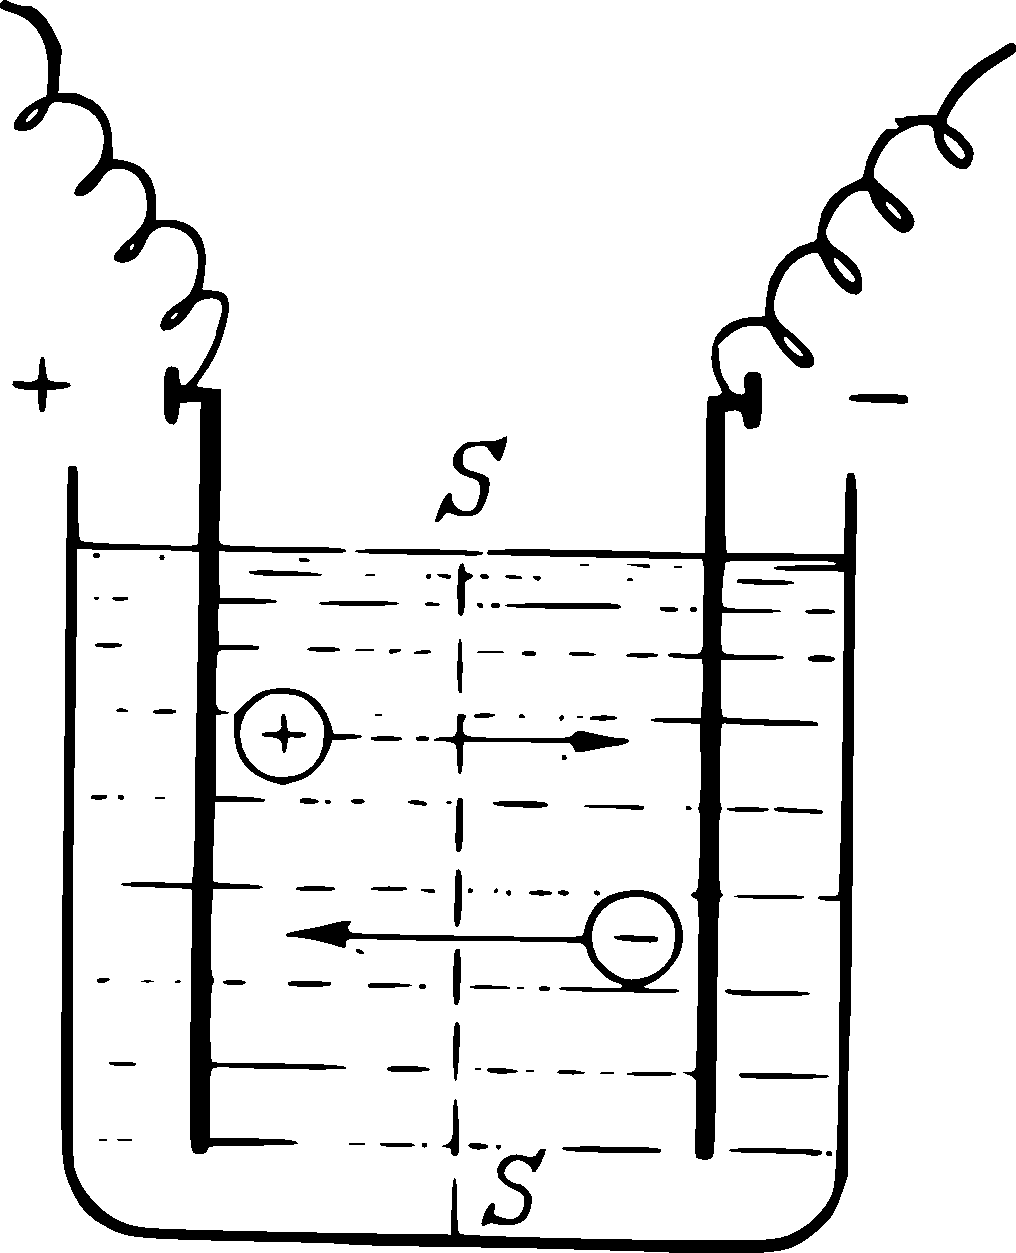
\includegraphics[width=0.8\textwidth]{figs/ch-22/fig-22-01.pdf}
\sidecaption{Current density in a conducting liquid.\zhcap{导电液体中的电流密度。}\label{fig-22-01}}
\end{marginfigure}

\subsection{}\label{22.3.1} The current density $\vb{j}$ \ssect{20.2.3} in an arbitrary section $SS$, perpendicular to the direction of ion motion (\figr{fig-22-01}), is equal to the sum of the current densities of the positive and negative ions:
\zhpar{垂直于离子运动方向的任一截面 $SS$（见\figr{fig-22-01}）上的电流密度 $\vb{j}$\ssect{20.2.3}，等于正、负离子电流密度之和，如下式所示。}
\begin{equation*}%
\vb{j} = \vb{j}_{+} + \vb{j}_{-}.
\end{equation*}
Here $\vb{j}_{+} = q_{+}n_{0+} \expval{\vb{v}_{+}}$ and $\vb{j}_{-} = q_{-}n_{0-} \expval{\vb{v}_{-}}$, where $q_{+}$ and $q_{-}$, $n_{0+}$ and $n_{0-}$, and $\expval{\vb{v}_{+}}$ and $\expval{\vb{v}_{-}}$ are the charges, concentrations and average velocities of ordered motion (\redem{drift} due in the action of the electric held) of the positive and negative ions. 
\zhpar{式中 $q_{+}$ 与 $q_{-}$、$n_{0+}$ 与 $n_{0-}$、$\expval{\vb{v}_{+}}$ 与 $\expval{\vb{v}_{-}}$ 分别为正、负离子的电荷、浓度和定向运动的平均速度（在外电场作用下的\redem{漂移}速度）。}

\subsection{}\label{22.3.2} The average velocities of ion drift are proportional to the electric field strength $\vb{E}$:
\zhpar{离子漂移的平均速度与电场强度 $\vb{E}$ 成正比，其关系如下式所示。}
\begin{align*}%
\expval{\vb{v}_{\perp}} & = u_{+}\vb{E}\,\, \text{and},\\
\expval{\vb{v}_{\parallel}} & = - u_{-}\vb{E},
\end{align*}
where $u_{+}$ and $u_{-}$ are the \redem{mobilities} of the positive and negative \redem{ions}. The mobility of an ion is equal to the ratio of the magnitude of the
average drift velocity vector to that of the field strength vector. The mobility is independent of the field strength vector $\vb{E}$. Since there are no bulk charges in electrolytes, $q_{+}n_{0+} + q_{-}n_{0-} = 0$. Moreover, $q_{+} = ez_{+} = \dfrac{F}{N_{A}}z_{+}$ \ssect{22.2.2}.
\zhpar{式中 $u_{+}$ 与 $u_{-}$ 分别为正、负\redem{离子}的\redem{迁移率}。离子的迁移率等于其平均漂移速度矢量的大小与电场强度矢量大小之比，且与电场强度无关。由于电解质中不存在体电荷，有 $q_{+}n_{0+} + q_{-}n_{0-} = 0$。此外，$q_{+}$ 由\ssect{22.2.2}给出。}

\subsection{}\label{22.3.3} \redem{Ohm's law of current density in electrolytes} (cf. \ssect{20.3.4}) is:
\zhpar{电解质中电流密度的\redem{欧姆定律}（参见\ssect{20.3.4}）如下式所示。}
\begin{equation*}%
\vb{j} = \frac{F}{N_{A}}z_{+}n_{0+} (u_{+} + u_{-})\vb{E}.
\end{equation*}
The resistivity $\rho$ of an electrolyte \ssect{20.3.4} is equal to
\zhpar{电解质的电阻率 $\rho$\ssect{20.3.4}由下式给出。}
\begin{equation*}%
\rho = \frac{N_{A}}{Fz_{+}n_{0+} (u_{+} + u_{-})}.
\end{equation*}
If a molecule of the solute dissociates into $k_{+}$ positive and $k_{-}$ negative ions, then
\zhpar{若溶质分子电离为 $k_{+}$ 个正离子和 $k_{-}$ 个负离子，则有如下关系。}
\begin{equation*}%
k_{+}z_{+} = k_{-}z_{-}; \quad n_{0+} = k_{+}\alpha n_{0} \qand n_{0-} = k_{-}\alpha n_{0},
\end{equation*}
where $\alpha$ is the degree of dissociation, $n_{0}$ is the concentration of the solute \ssect{22.1.5} and
\zhpar{式中 $\alpha$ 为电离度，$n_{0}$ 为溶质的浓度\ssect{22.1.5}，此时电阻率可写为如下形式。}
\begin{equation*}%
\rho = \frac{N_{A}}{Fz_{+}k_{+}\alpha n_{0} (u_{+} + u_{-})}.
\end{equation*}
The ratio $N_{A}/z_{+}$ is the number of positive ions in one gram equivalent \ssect{22.1.4}. We introduce the quantity
\zhpar{比值 $N_{A}/z_{+}$ 即一克当量中正离子的个数\ssect{22.1.4}。为此引入如下物理量。}
\begin{equation*}%
C = \frac{k_{+}n_{0}z_{+}}{N_{A}} = \frac{k_{-}n_{0}z_{-}}{N_{A}},
\end{equation*}
which is called the \redem{equivalent concentration of the solution}. It is the number of gram equivalents of the ions of one sign contained in unit volume of the electrolyte (either in the free state or bound in the molecules). Then
\zhpar{上式所定义的量称为溶液的\redem{当量浓度}，它是单位体积电解质中同一符号离子（无论是自由状态还是结合在分子中）所含的克当量数。于是电阻率可写为如下形式。}
\begin{equation*}%
\rho = \frac{1}{F C \alpha(u_{+} + u_{-})}.
\end{equation*}


\section{Electrical Conduction in Gases}
\label{sec-22.4}
\zhtitle{气体中的导电}


\subsection{}\label{22.4.1} Gases, consisting of neutral atoms and molecules, are insulators and do not conduct an electric current. Gases arc capable of conduction after they are ionized.
\zhpar{由中性原子和分子组成的气体是绝缘体，不导电。只有在电离之后，气体才能导电。}

The \redem{ionization of a molecule} (or \redem{atom}) consists in the detachment of one or several electrons, after which the molecule (or atom) is converted into a positive ion. If a molecule (or atom) gains electrons, it becomes a negative ion.
The reverse process, in which electrons join a positive ion to form a neutral molecule (or atom), is called \redem{recombination}. 
\zhpar{分子（或原子）的\redem{电离}是指分离出一个或几个电子，使分子（或原子）变为正离子；若分子（或原子）获得电子，则变为负离子。其逆过程，即电子与正离子结合形成中性分子（或原子），称为\redem{复合}。}

\subsection{}\label{22.4.2} To ionize a molecule (or atom) it is necessary to perform the \redem{work of ionization} $W_{i}$ to overcome the forces of attraction between the electron being detached and the other particles of the molecule (or atom). The work $W_{i}$ depends upon the energy state of the electron being detached \ssect{39.1.9} in the atom or molecule of the given gas. The ionization energy increases with the electron detachment factor, i.e. with the number of electrons detached from each atom.
\zhpar{要使分子（或原子）电离，必须做\redem{电离功} $W_{i}$，以克服被移出的电子与分子（或原子）中其他粒子之间的吸引力。电离功 $W_{i}$ 取决于气体中被移出电子所处的能量状态\ssect{39.1.9}。电离能随电子移出程度（即每个原子被移出的电子数）的增加而增大。}

\subsection{}\label{22.4.3} The \redem{ionization potential} $V_{i}$ is the potential difference that the charged particle must traverse in an accelerating electric held in order to accumulate energy equal to the work of ionization $W_{i}$. Thus $V_{i} = W_{i}/e$, where $e$ is the magnitude of the charge of the particle.
\zhpar{\redem{电离电势} $V_{i}$ 是带电粒子在加速电场中所经过的电势差，粒子借此获得等于电离功 $W_{i}$ 的能量。因此 $V_{i} = W_{i}/e$，其中 $e$ 为粒子电荷的大小。}

\subsection{}\label{22.4.4} A gas is ionized by external effects: raising the temperature sufficiently, the action of various kinds of radiation, cosmic radiation, bombardment of the molecules (or atoms) of the gas by high-speed electrons or ions, etc. The \redem{intensity}, or \redem{rate, of ionization} is measured by the number of pairs of particles of opposite sign formed in unit time in unit volume of the gas. 
\zhpar{气体可由外部因素电离，如充分升高温度、各种辐射（包括宇宙射线）的作用，以及高速电子或离子轰击气体分子（或原子）等。电离的\redem{强度}，或称电离\redem{速率}，以单位时间内单位体积气体中产生的异号粒子对数来度量。}

\subsection{}\label{22.4.5} \redem{Collision ionization} is the process in which a gas is ionized by the action of fast-moving electrons or by ions. The minimum kinetic energy \ssect{3.2.1} that an ionizing particle must have is assessed by applying the laws of conservation of momentum and energy. Thus
\zhpar{\redem{碰撞电离}是指气体在快速运动的电子或离子作用下发生电离的过程。应用动量守恒定律和能量守恒定律，可求出电离粒子所需具有的最小动能\ssect{3.2.1}，其关系如下式所示。}
\begin{equation*}%
\frac{mv^{2}}{2} = W_{i} \, \left( 1 + \frac{m}{M}\right)
\end{equation*}
where $W_{i}$ is the work of ionization, $m$ is the mass of the electron and $M$ is the mass of the atom.
\zhpar{式中 $W_{i}$ 为电离功，$m$ 为电子质量，$M$ 为原子质量。}

The smaller the ratio $m/M$, the closer this energy is to $W_{i}$. An electron and a single-charge ion accumulate the same energy $E =e \, \Delta V$ if they traverse the same potential difference $\Delta V$.
\zhpar{比值 $m/M$ 越小，该能量就越接近 $W_{i}$。若电子与带单位电荷的离子经过相同的电势差 $\Delta V$，则获得相同的能量 $E =e \, \Delta V$。}

It follows from the preceding formula that for collision ionization by electrons and ions, the latter of a mass \num{d4} times that of the electron, ions must travel across a greater potential difference in an accelerating field than electrons.
\zhpar{由上式可知，对于电子和离子引起的碰撞电离，若离子的质量为电子质量的 \num{d4} 倍，则离子在加速电场中必须经过比电子更大的电势差。}

\section{Various Types of Gas Discharges}
\label{sec-22.5}
\zhtitle{各种类型的气体放电}

\subsection{}\label{22.5.1} A \redem{gas discharge} is the process of current conduction through a gas.
\zhpar{\redem{气体放电}是指电流通过气体导电的过程。}


\begin{marginfigure}[-3cm]
\centering
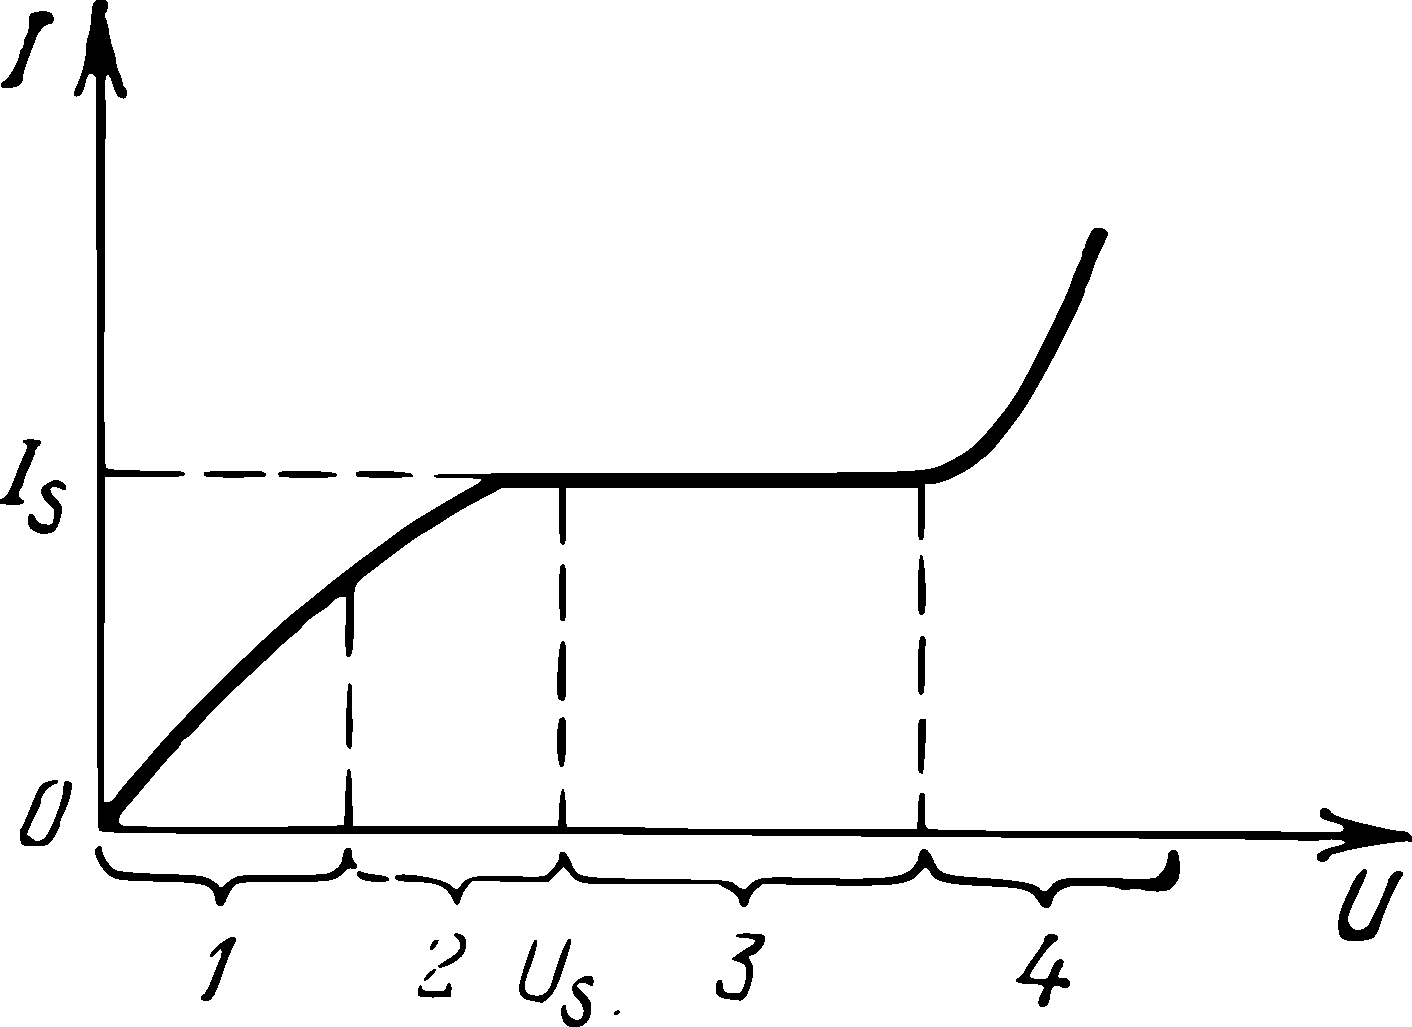
\includegraphics[width=0.8\textwidth]{figs/ch-22/fig-22-02.pdf}
\sidecaption{Current-voltage relationship in a semi-self-maintained discharge gas.\zhcap{半自持气体放电中的电流-电压关系。}\label{fig-22-02}}
\end{marginfigure}


A \redem{semi-self-maintained gas discharge} is one caused by external ionizing agents \ssect{22.4.4} and ceasing when the ionizing action stops. The curve in \figr{fig-22-02} shows the dependence of the current $I$ in a semi-self-maintained discharge on the voltage $U$ across the electrodes, in the 1st region of the curve, at low voltages, Ohm's law, similar to the one for electrolytes \ssect{22.3.3}, is valid. If electrons and monovalent ions are formed in the gas, then
\zhpar{\redem{半自持气体放电}是由外部电离因素引起的放电，外部电离作用停止时放电也随之停止。\figr{fig-22-02}中的曲线给出了半自持放电中电流 $I$ 与电极间电压 $U$ 的关系。在第一区段（低电压）内，与电解质的情形类似\ssect{22.3.3}，欧姆定律成立。若气体中形成了电子和一价离子，则有如下关系。}
\begin{equation*}%
\vb{j} = en_{0}(u_{+} + u_{-} ) \vb{E},
\end{equation*}
where $n_{0}$ is the number of pairs of oppositely charged particles in unit volume, $u_{+}$ and $u_{-}$ are the mobilities of the positive and negative ions, and $e$ is the magnitude of the charge of the electron. In a wide pressure range, from 10 to \SI{d7}{\pascal}, the mo­bility of gaseous ions is inversely proportional to the pressure.
\zhpar{式中 $n_{0}$ 为单位体积中带相反电荷的粒子对数，$u_{+}$ 与 $u_{-}$ 分别为正、负离子的迁移率，$e$ 为电子电荷的大小。在从 10 到 \SI{d7}{\pascal} 的宽广压强范围内，气体离子的迁移率与压强成反比。}

\subsection{}\label{22.5.2} The relation between the current $I$ and the voltage $U$ is no longer linear in the 2nd region of the curve in \figr{fig-22-02} because the ion concentration decreases in the gas. In this region $U$ the current increases slower and slower with an increase in $U$.
\zhpar{在曲线的第二区段（见\figr{fig-22-02}）中，由于气体中离子浓度降低，电流与电压不再呈线性关系。在此区段中，随 $U$ 增大，电流的增长越来越慢。}

Beginning with a certain voltage $U_{s}$, the current re­ mains constant in the 3rd
region of the curve in \figr{fig-22-02} when the voltage is in­ creased. This occurs because, at a constant rate of ionization \ssect{22.4.4} in strong electric fields, all the ions formed in unit time in the gas reach the electrodes. No further increase in the current takes place at a fixed rate of ionization. Saturation results because all the charged particles produced in the gas travel in a strong electric field and reach the electrodes before an appreciable part of them have enough time to recombine with particles of opposite charge.
\zhpar{当电压增大到某一值 $U_{s}$ 以后，在曲线的第三区段（见\figr{fig-22-02}）中，电流不再随电压增大而增加。这是因为在强电场中，给定电离速率下气体中单位时间内产生的所有离子都能到达电极，因此在电离速率固定时，电流不会继续增大。饱和现象的原因是：气体中产生的全部带电粒子在强电场中运动，在其中相当一部分粒子有足够时间与异号电荷复合之前，就已到达电极。}

The saturation current $U_{s}$ is the maximum current that can be obtained at a given rate (intensity) of ionization:
\zhpar{饱和电流 $U_{s}$ 是在给定电离速率（强度）下能够获得的最大电流，其表达式如下。}
\begin{equation*}%
I_{s} = eN_{0}
\end{equation*}
where $N_{0}$ is the maximum number of pairs of monovalent ions formed in the gas in unit time at a given rate of ionization. The linear relation between $I_{s}$ and $N_{0}$ confirms the ionic nature of electrical conduction in gases.
\zhpar{式中 $N_{0}$ 为在给定电离速率下，气体中单位时间内形成的一价离子对的最大数目。$I_{s}$ 与 $N_{0}$ 之间的线性关系证实了气体中导电的离子本性。}

\subsection{}\label{22.5.3} A \redem{self-maintained gas discharge} is one that continues after the action of the external ionizing agent ceases. To obtain such a discharge it is necessary for new pairs of oppositely charged particles to be formed continuously in the gas. The main source of these particles is collision ionization \ssect{22.4.5}. At a certain sufficiently high voltage across the electrodes, the electrons are so highly accelerated by the electric held that their energy proves adequate to ionize the gas molecules \ssect{22.4.5}. This is called \redem{volume ionization}. Secondary electrons, accelerated in the electric held, also ionize the gas molecules. As a result, the number of current carriers in the gas and its electrical conductance are greatly increased (4th region in \figr{fig-22-02}. But, by itself, ionization by the action of electrons is insufficient to produce a self-maintained discharge. 
\zhpar{\redem{自持气体放电}是指外部电离因素停止作用后仍能持续的放电。要维持这种放电，气体中必须持续产生新的带相反电荷的粒子对，其主要来源是碰撞电离\ssect{22.4.5}。在电极间电压足够高时，电子在电场中被加速，获得的能量足以使气体分子电离，这称为\redem{体积电离}。二次电子在电场中加速后也能使气体分子电离。结果，气体中的载流子数目及其电导率大大增加（见\figr{fig-22-02}中的第四区段）。但是，仅靠电子引起的电离不足以维持自持放电。}

Electrons travelling in the direction from the cathode toward the anode ionize the molecules of gas located closer to the anode than the place where the electrons are unitied. If the energy of the positive ions is insufficient for collision ionization of the gas molecules or for knocking electrons out of the metallic cathode (\redem{surface ionization}), electrons can be produced near the cathode of a gas-discharge tube only by external ionizing agents. When the action of these agents is- stopped, the region of collision ionization by electrons contracts toward the anode as the electrons move in this direction. Under these conditions the gas discharge is extinguished as soon as collision ionization ceases. 
\zhpar{从阴极向阳极运动的电子，使位于比电子产生处更靠近阳极的气体分子电离。若正离子的能量不足以使气体分子碰撞电离，或不足以从金属阴极中击出电子（\redem{表面电离}），那么在气体放电管的阴极附近，只能依靠外部电离因素产生电子。外部作用停止后，随着电子向阳极运动，电子碰撞电离区域向阳极收缩。在这种条件下，一旦碰撞电离停止，气体放电就会熄灭。}

\subsection{}\label{22.5.4} Surface ionization \ssect{22.5.3}, initiated at high voltage $U$, produces secondary electrons and sets up a two-way avalanche of electrons and positive ions. After this the action of the external ionizing agent is no longer essential for continuing the gas discharge. When the voltage $U$ across the electrodes of a gas-discharge tube is raised sufficiently, an \redem{electric breakdown of the gas} occurs. This is the transition from a semi-self-maintained to a self-maintained gas discharge. The voltage $U = U_{bd}$, corresponding to electric breakdown, is called the \redem{ignition potential}, or \redem{breakdown voltage}. The breakdown voltage for a gas discharge in a tube having flat parallel electrodes at the distance $d$ from each other depends upon the product $pd$, where $p$ is the gas pressure \figr{fig-22-03}. In addition, depends on the chemical nature of the gas and the material of the cathode.
\zhpar{在高电压 $U$ 下开始的表面电离（见\ssect{22.5.3}）产生二次电子，并形成电子与正离子的双向雪崩。此后，气体放电的维持不再依赖外部电离因素。当气体放电管电极间的电压 $U$ 升高到足够大时，发生\redem{气体的电击穿}，即由半自持放电转变为自持放电。与电击穿相应的电压 $U = U_{bd}$ 称为\redem{着火电势}或\redem{击穿电压}。对于两平行平板电极相距为 $d$ 的气体放电管，击穿电压取决于乘积 $pd$，其中 $p$ 为气体压强（见\figr{fig-22-03}）。此外，击穿电压还与气体的化学性质及阴极材料有关。}
\begin{marginfigure}[-3cm]
\centering
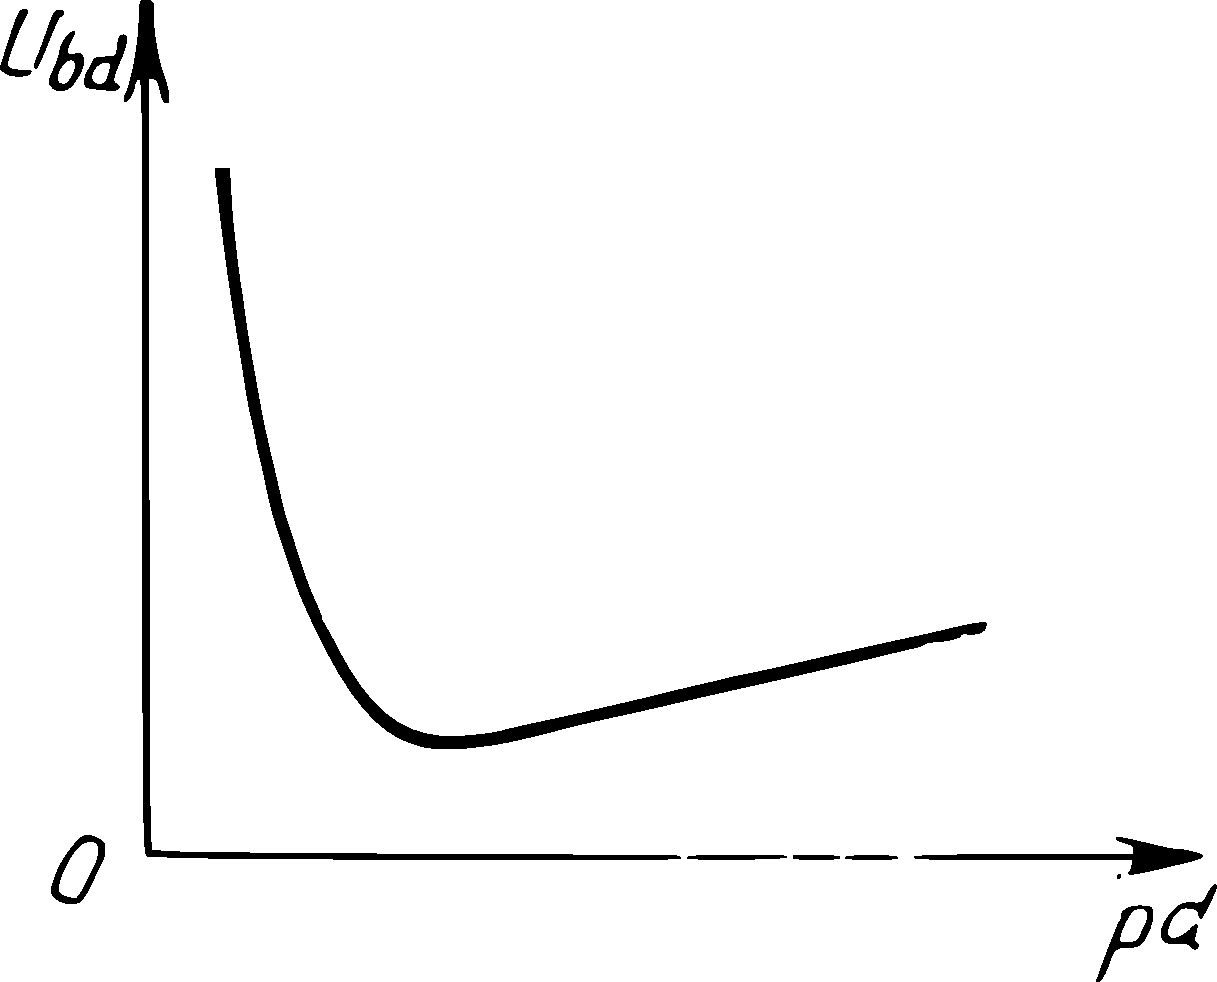
\includegraphics[width=0.8\textwidth]{figs/ch-22/fig-22-03.pdf}
\sidecaption{The breakdown voltage for gas discharge.\zhcap{气体放电的击穿电压。}\label{fig-22-03}}
\end{marginfigure}

Self-maintained gas discharges are classified into glow, corona, spark and arc discharges. They are not discussed in the present handbook.
\zhpar{自持气体放电可分为辉光放电、电晕放电、火花放电和电弧放电。本手册不讨论这些放电。}

\section{Certain Information on Plasma}
\label{sec-22.6}
\zhtitle{关于等离子体的若干知识}

\subsection{}\label{22.6.1} \redem{Plasma} is a special state of matter, whose most important property is a predominant, or even complete, ionization of the particles of matter. The \redem{degree of ionization} $\alpha$ is the ratio of the number of ionized particles to their initial number. Plasma is classified as \redem{weakly ionized} (when $\alpha$ is a fraction of one percent), \redem{moderately ionized} (when $\alpha$ equals several percent) and \redem{fully ionized} (when $\alpha$ is close to 100 per cent).
\zhpar{\redem{等离子体}是物质的一种特殊状态，其最重要的特征是物质粒子的高度电离，甚至是完全电离。\redem{电离度} $\alpha$ 是电离粒子数与初始粒子数之比。按电离程度，等离子体可分为\redem{弱电离}（$\alpha$ 不足百分之一）、\redem{中等电离}（$\alpha$ 为百分之几）和\redem{完全电离}（$\alpha$ 接近 100\%）三类。}

Weakly ionized plasma is found in the \redem{ionosphere}, the conducting layer of the atmosphere. The ionosphere extends from 60 to \SI{2d4}{\kilo\meter} above the earth's surface.
\zhpar{弱电离等离子体存在于电离层中，电离层是大气中的导电层。电离层从地球表面向上延伸，高度为 60 至 \SI{2d4}{\kilo\meter}。}

Fully ionized plasma, formed at ultra-high temperatures (high-temperature plasma), exists on the sun and hot stars. Under laboratory conditions, plasma is produced in gas discharges \ssect{22.5.1} and gaseous-discharge lamps. Accelerated plasma is employed as the working medium \ssect{11.1.1} in jet engines. Plasma can also be used for the direct conversion of internal energy into electrical energy (magnetohydrodynamic generators and plasma sources of electrical energy).
\zhpar{完全电离的等离子体在超高温（高温等离子体）条件下形成，存在于太阳和炽热的恒星上。在实验室条件下，等离子体可在气体放电及气体放电灯中产生。加速的等离子体用作喷气发动机的工作介质\ssect{11.1.1}。等离子体还可直接将内能转换为电能（磁流体发电机和等离子体电源）。}

The great number of charged particles in a plasma provides for its high electrical conductance; in this aspect its properties approach those of conductors of electric current.
\zhpar{等离子体中大量的带电粒子使其具有很高的电导率；就这一点而言，等离子体的性质接近于导体。}

\subsection{}\label{22.6.2} A condition for the existence of a plasma is a certain minimum density $\rho_{\text{min}}$ of charged particles. Beginning with this density, we can speak of a plasma rather than a simple accumulation of separate charged particles. The density $\rho_{\text{min}}$ is determined by the inequality $L \gg D$, where $L$ is a linear dimension of the system of charged particles and $D$ is a typical ``plasma'' parameter, the length called the \redem{Debye-H\"uckel screening} radius (it is also called the \redem{Debye shielding length} or \redem{Debye length}):
\zhpar{等离子体存在的条件是带电粒子具有一定的最小密度 $\rho_{\text{min}}$。达到这一密度时，我们才能将其称为等离子体，而不是分散的带电粒子的简单集合。密度 $\rho_{\text{min}}$ 由不等式 $L \gg D$ 确定，其中 $L$ 为带电粒子系统的线度，$D$ 为典型的“等离子体”参数，即\redem{德拜-休克尔屏蔽}半径（亦称\redem{德拜屏蔽长度}或\redem{德拜长度}），其表达式如下。}
\begin{align*}%
D & = \left( \sum_{i} \frac{4 \pi q_{i}^{2}n_{i}}{k T_{i}} \right)^{-1/2} && \text{(in cgse units),}\\
D & = \left( \sum_{i} \frac{ q_{i}^{2}n_{i}}{\varepsilon_{0} k T_{i}} \right)^{-1/2} && \text{(in SI units),}
\end{align*}
where $q_{i}$ is the charge of the $i$-th species of particles, $n_{i}$ is their concentration, $T_{i}$ is their temperature, $k$ is Boltzmann's constant \ssect{8.4.5} and $\varepsilon_{0}$ is the electric constant. Summation is to be carried out over all the species of particles. The quantity $D$ is the distance over which the Coulomb field of any charge of the plasma is shielded. The shielding occurs because any charge is predominantly surrounded by oppositely charged particles. 
\zhpar{式中 $q_{i}$ 为第 $i$ 种粒子的电荷，$n_{i}$ 为其浓度，$T_{i}$ 为其温度，$k$ 为玻尔兹曼常量\ssect{8.4.5}，$\varepsilon_{0}$ 为真空电容率。求和遍及所有种类的粒子。量 $D$ 是等离子体中任一电荷的库仑场被屏蔽的距离。屏蔽之所以发生，是因为任一电荷周围主要被异号带电粒子所包围。}

According to a more exact definition, a plasma is a quasi­ neutral assembly of a large number of charged particles that occupy a region of space with the linear dimensions $L \gg D$. The violation of quasi-neutrality in the plasma is eliminated by the strong electric fields set up in it. 
\zhpar{按照更精确的定义，等离子体是线度 $L \gg D$ 的空间区域中大量带电粒子组成的准中性集合体。等离子体中准中性的破坏，会被其内部建立的强电场所消除。}

The Debye-H\"uckel screening radius characterizes the interaction of the particles in the plasma. It was found that $E_{p}/E_{k} \propto N^{2/3}$, where $N = 4\pi n D^{3}/3$. Here $E_{p}$ is the potential energy of interaction between two particles located at an average distance of $n^{-1/3}$ from each other ($n$ being the concentration of particles), and $E_{k}$ is the kinetic energy of these particles. The quantity $N$ is the total number of charged particles inside a sphere of radius $D$, and is called the \redem{Debye number}. If $N$ is large, the plasma is said to be \redem{gaseous} and can be dealt with thermodynamically as an ideal gas with the state equation $p = nkT$ \ssect{8.4.5}.
\zhpar{德拜-休克尔屏蔽半径表征了等离子体中粒子间的相互作用。研究表明 $E_{p}/E_{k} \propto N^{2/3}$，其中 $N = 4\pi n D^{3}/3$。这里 $E_{p}$ 为两粒子平均间距为 $n^{-1/3}$（$n$ 为粒子浓度）时的相互作用势能，$E_{k}$ 为这些粒子的动能。量 $N$ 为半径为 $D$ 的球体内带电粒子的总数，称为\redem{德拜数}。若 $N$ 很大，则称该等离子体为\redem{气态等离子体}，可以作为满足物态方程 $p = nkT$ 的理想气体进行热力学处理\ssect{8.4.5}。}

\subsection{}\label{22.6.3} Coulomb long-range interaction of charged particles in a plasma leads to its qualitative uniqueness that enables it to be regarded as a special, \redem{fourth state of aggregation of matter. The most important properties of plasma} are:
\zhpar{等离子体中带电粒子间的库仑长程相互作用，使其具有独特的性质，因此可以将其视为一种特殊的\redem{物质的第四种聚集态}。\redem{等离子体的最重要性质}是：}
\begin{enumerate}[label = (\alph*)]
\item its strong interaction, due to its high electrical conduction, with external magnetic and electric fields;
\zhpar{由于其高电导率，它与外部磁场和电场有强烈的相互作用；}
\item specific collective interaction of particles in the plasma (by means of a special held whose nature and origin is beyond the scope of this handbook);
\zhpar{等离子体中粒子之间特有的集体相互作用（借助某种特殊的场实现，该场的性质和起源超出本手册的范围）；}
\item the fact that due to long-range interaction it is a special kind of elastic medium in which various types of vibrations and waves can be readily excited and propagated.
\zhpar{由于长程相互作用，它是一种特殊的弹性介质，其中各种振动和波动都很容易被激发和传播。}
\end{enumerate}
\subsection{}\label{22.6.4} The motion of plasma in a magnetic held is employed to directly convert the internal energy of an ionized gas into electrical energy. This method is made use of in a \redem{magneto-hydrodynamic (MHD) generator}. This generator operates as follows: gas produced in the combustion of fuel and constituting a plasma passes through a strong traverse magnetic held. In a conducting plasma, as in any conductor moving in such a held, electromagnetic induction \ssect{24.1.1} occurs. The induced emf can be taken off by means of electrodes in the external circuit. A schematic diagram of an MHD generator is shown in \figr{fig-22-04}.
\zhpar{等离子体在磁场中的运动可用来直接将电离气体的内能转换为电能。这一方法应用于\redem{磁流体（MHD）发电机}。其工作原理如下：燃料燃烧产生的、构成等离子体的气体，通过强横向磁场。在导电的等离子体中，正如任何在这种磁场中运动的导体那样，会发生电磁感应\ssect{24.1.1}。感应电动势可通过电极引到外电路中。磁流体发电机的示意图如\figr{fig-22-04}所示。}


\begin{marginfigure}[-2cm]
\centering
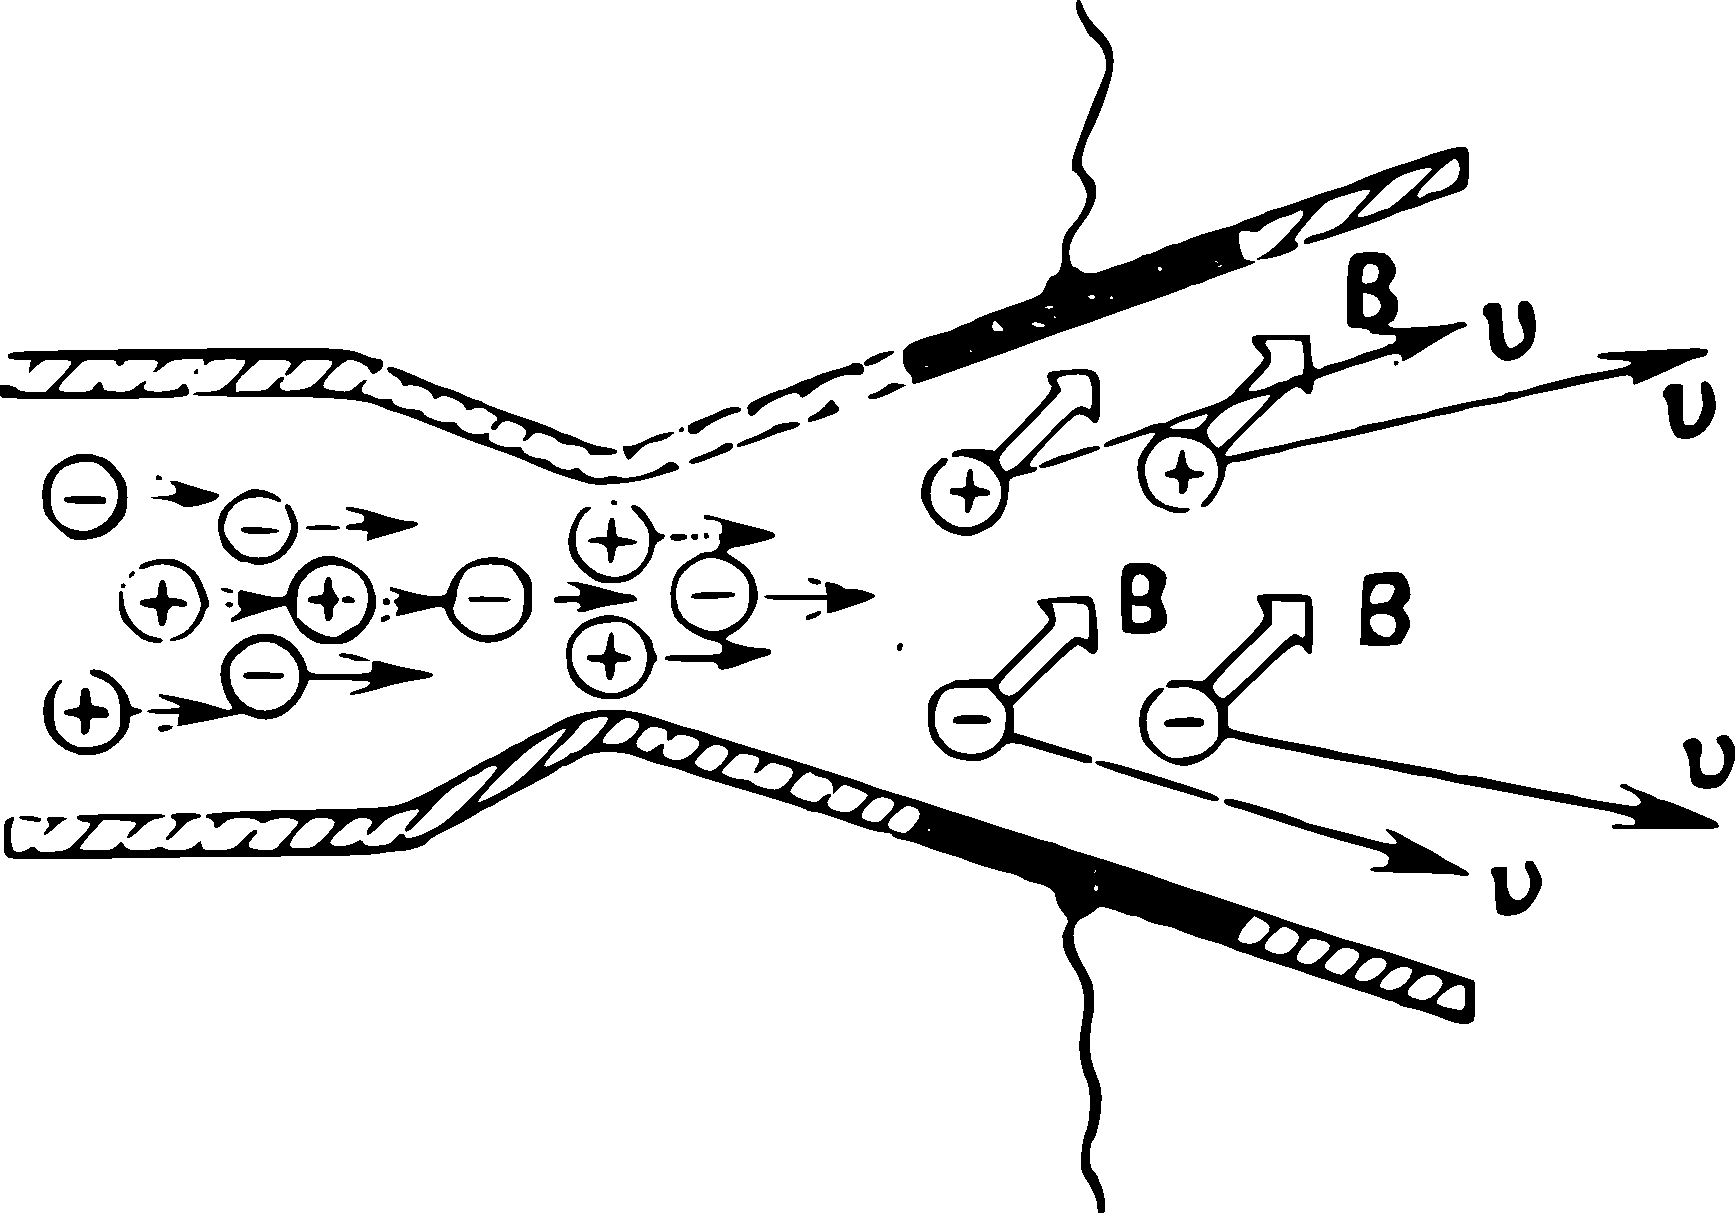
\includegraphics[width=\textwidth]{figs/ch-22/fig-22-04.pdf}
\sidecaption{ A schematic diagram of an MHD generator.\zhcap{磁流体发电机的示意图。}\label{fig-22-04}}
\end{marginfigure}



The ionized gas produced in fuel combustion passes through the nozzle and its internal energy is converted into kinetic energy. As this gas passes through the transverse magnetic field $\vb{B}$, the positive ions move toward the upper electrode by the action of the induced electric held \ssect{24.1.1} and the free electrons move toward the lower electrode. When we connect the electrodes to an external load, a current is obtained in the circuit. 
\zhpar{燃料燃烧产生的电离气体流过喷管，其内能转换为动能。当该气体通过横向磁场 $\vb{B}$ 时，在感应电场\ssect{24.1.1}作用下，正离子向上方电极运动，自由电子向下方电极运动。将电极接入外部负载后，电路中便有电流通过。}

\subsection{}\label{22.6.5} A state of thermodynamic equilibrium is possible at a definite temperature in the plasma when the loss of charged particles due to recombination \ssect{22.4.1} is recompensed by new acts of ionization. The average kinetic energies of the various particles making up such a plasma are the same. The processes of energy exchange between the particles of this plasma, as well as the energy exchange of the plasma with blackbody radiation \ssect{36.1.8} are equilibrium processes \ssect{8.3.7}. A \redem{plasma} with the aforesaid properties is said to be \redem{isothermal}. It exists in the atmospheres of high-temperature stars.
\zhpar{若在确定温度下，等离子体中因复合而损失的带电粒子能被新的电离过程所补偿，则等离子体可以处于热力学平衡状态。这种等离子体中各种粒子的平均动能相同。等离子体内部的能量交换过程，以及等离子体与黑体辐射之间的能量交换\ssect{36.1.8}，均为平衡过程\ssect{8.3.7}。具有上述性质的\redem{等离子体}称为\redem{等温等离子体}。这种等离子体存在于高温恒星的大气中。}

A condition required for a high degree of ionization of a thermodynamically equilibrium plasma, consisting of two kinds of charged particles, equal in magnitude and opposite in sign, is the maximum reduction in the recombination \ssect{22.4.1} of the particles. A completely ionized plasma can be obtained at $kT \gg eV_{i}$ where $V_{i}$ is the ionization potential \ssect{22.4.3} of the gas atoms and $kT$ is the average energy of thermal motion of the plasma particles. For hydrogen and deuterium this corresponds to $T \approx  \SI{160000}{\kelvin}$. Essential under these conditions are the radiation of the plasma and the difficulty of isolating the plasma from the walls of its container \ssect{22.6.7}.
\zhpar{对于由两种等量异号带电粒子组成的热力学平衡等离子体，要获得高度电离，其条件是使粒子的复合减至最少。当 $kT \gg eV_{i}$ 时可获得完全电离的等离子体，其中 $V_{i}$ 为气体原子的电离电势\ssect{22.4.3}，$kT$ 为等离子体粒子热运动的平均能量。对于氢和氘，这相当于 $T \approx \SI{160000}{\kelvin}$。在这些条件下，需要重视的问题有：等离子体的辐射，以及将等离子体与容器壁隔离的困难\ssect{22.6.7}。}

\subsection{}\label{22.6.6} In the plasma of a gas discharge \ssect{22.5.1} (\redem{gas-discharge plasma}) thermodynamical equilibrium \ssect{22.6.5} is absent. The charged particles of such a plasma are in an accelerating electric field.
\zhpar{在气体放电的等离子体\ssect{22.5.1}（\redem{气体放电等离子体}）中，不存在热力学平衡\ssect{22.6.5}。这种等离子体的带电粒子处于加速电场之中。}

The average kinetic energy of the electrons in a gas-discharge plasma is characterized by a certain \redem{electron temperature} $T_{e}$ corresponding to the Maxwellian energy distribution of the electrons \ssect{10.3.7}. Owing to the lack of thermodynamical equilibrium in such a plasma, $T_{e}$ is of a conventional nature. The average kinetic energy of the neutral particles is substantially less than that of the electrons. Besides the electron temperature $T_{e}$, the parameters of a gas-discharge plasma are: the electron concentration $n_{e}$, the number of ionizations per electron per second, the density of the ion or electron current, and the longitudinal electric field strength $E_{z}$ established along the symmetry axis of the plasma.
\zhpar{气体放电等离子体中电子的平均动能，可用一个确定的\redem{电子温度} $T_{e}$ 来表征，它对应于电子的麦克斯韦能量分布\ssect{10.3.7}。由于该等离子体不存在热力学平衡，$T_{e}$ 具有约定的性质。中性粒子的平均动能远小于电子的平均动能。除电子温度 $T_{e}$ 外，气体放电等离子体的参数还包括：电子浓度 $n_{e}$、每个电子每秒的电离次数、离子或电子电流密度，以及沿等离子体对称轴建立的纵向电场强度 $E_{z}$。}

\subsection{}\label{22.6.7} The existence of a thermodynamically nonequilibrium gas-discharge plasma is made possible by the energy of the discharge current passing through it. In the absence of an external electric field, the gas-discharge plasma disappears.
\zhpar{热力学非平衡的气体放电等离子体之所以能够存在，是由于流经其中的放电电流所携带的能量。若没有外电场，气体放电等离子体就会消失。}

The disappearance of an unmaintained gas-discharge plasma that has been left to Itself is called \redem{deionization of the gas}.
\zhpar{无外部维持、任其自行消失的气体放电等离子体的消失过程，称为\redem{气体的去电离}。}

In addition to the ionization and recombination processes \ssect{22.4.1}, a large share of the energy balance of a plasma that exists in a limited volume consists in the interaction between the plasma and the walls confining its volume, as well as the radiation of the plasma and the transport of radiation in it. The diffusion of the charged particles to the walls and their recombination on the walls, and the transfer of energy to the walls by heat conduction \ssect{10.8.2} contaminate the plasma with impurities and reduce its energy. To avoid these phenomena, measures are taken to confine the plasma by a magnetic field to prevent contact with the walls.
\zhpar{除电离和复合过程外，对于限制在有限体积内的等离子体，其能量平衡中很大一部分取决于等离子体与限制其体积的器壁之间的相互作用，以及等离子体的辐射和辐射在其中的输运。带电粒子向器壁扩散并在器壁上复合，以及通过热传导将能量传给器壁\ssect{10.8.2}，都会使等离子体受到杂质污染并降低其能量。为避免这些现象，人们采取措施用磁场约束等离子体，使其不与器壁接触。}

Radiation of the plasma in the optical range and in the far ultraviolet consists of: braking radiation (bremsstrahlung) of the electrons that occurs when they are retarded by the ions, ordinary radiation produced by excited particles, and recombination radiation that occurs in the recombination process
\ssect{22.4.1}. In a magnetic field, a plasma also has a special beta­ tron (synchrotron) radiation, which is beyond the scope of this handbook.
\zhpar{等离子体在光学波段和远紫外波段的辐射包括：电子被离子减速时产生的韧致辐射（轫致辐射），受激粒子产生的普通辐射，以及复合过程中产生的复合辐射\ssect{22.4.1}。在磁场中，等离子体还具有特殊的\redem{电子感应加速器辐射（同步辐射）}，这超出了本手册的范围。}